\documentclass[conference]{IEEEtran}
\IEEEoverridecommandlockouts
% The preceding line is only needed to identify funding in the first footnote. If that is unneeded, please comment it out.
\usepackage{cite}
\usepackage{amsmath,amssymb,amsfonts}
\usepackage{algorithmic}
\usepackage{graphicx}
\usepackage{textcomp}
\usepackage{xcolor}
\def\BibTeX{{\rm B\kern-.05em{\sc i\kern-.025em b}\kern-.08em
T\kern-.1667em\lower.7ex\hbox{E}\kern-.125emX}}
\begin{document}

\title{TaintBlade: A framework for automated protocol reverse engineering and study of botnet command and control protocols
}

\author{\IEEEauthorblockN{1\textsuperscript{st} Given Name Surname}
    \IEEEauthorblockA{\textit{dept. name of organizatiosn (of Aff.)} \\
        \textit{name of organization (of Aff.)}\\
        City, Country \\
        email address or ORCID}
    \and
    \IEEEauthorblockN{2\textsuperscript{nd} Given Name Surname}
    \IEEEauthorblockA{\textit{dept. name of organization (of Aff.)} \\
        \textit{name of organization (of Aff.)}\\
        City, Country \\
        email address or ORCID}
}

\maketitle

\begin{abstract}
    TODO redact this at the end
\end{abstract}

\begin{IEEEkeywords}
    TODO keywords
\end{IEEEkeywords}

\section{Introduction}
TODO - This section introduces the problem we are dealing with and motivates
the creation of this tool

\section{Background}

TODO - This section goes over the state of the art on analyzing malware
binaries, past work on protocol reverse engineering and available tools.

\section{Design}
TODO - This section covers the general structure of the tool and the different
modules and functionalities implemented.

- Requirements: overview and goals of the tool
- Arch: overview and details of each stage
- Implementation, with repo and how to use

\

In the previous sections, we introduced the issue of automating protocol
reverse engineering and the relevance of this task in the context of the
analysis of malware transmitting malicious communications. In this section, we
will now describe the automated protocol reverse engineering framework, called
\textit{TaintBlade}, that we have developed for tackling this task. Overall,
this tool pursues three main goals: (1) to perform message inference of the
underlying ingress protocol of a program, offering an accurate representation
of its compounding fields and the purpose of each byte; (2) to provide a
complete trace of the activities carried out by the instrumented program,
including a viewpoint into loaded images, child processes, executed routines
and their arguments, therefore helping the analyst with the reversing task,
rathering than just offering a black-box tool; (3) to become a framework usable
not only by malware analysts by offering specific functionalities aimed for
studying malware behaviours, but also by the general public by providing an
intuitive and fully enriched graphical user interface that offers additional
features and enhances cohesion over the data produced by the tool.

\subsection{Architecture overview}

\begin{figure}[htbp]
    \centerline{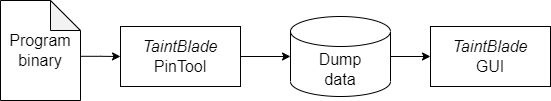
\includegraphics[width=0.9\columnwidth]{images/generalarch.drawio.png}}
    \caption{Example of a figure caption.}
    \label{fig_3_generalarch}
\end{figure}

From a general viewpoint, the functioning of \textit{TaintBlade} is, as shown
in figure \ref{fig_3_generalarch}: (1) the user selects a binary (an
executable) to be traced; (2) the program is executed and instrumented by
\textit{Intel PIN}, using \textit{TaintBlade} as a pintool, which reverses the
protocol of the program; (3) the pintool generates a set of output
\textit{.dfx} dump files and/or a SQLite database with all traced data; (4) the
user can navigate the resulting data by means of \textit{TaintBlade} GUI, which
interacts with the database, or by accessing the output dump files.

The \textit{TaintBlade} pintool is the central component of the framework. It
encompasses all the necessary instrumentation and tracing functionalities
required for the protocol reverse engineering task. At its core, the pintool
utilizes Intel PIN, which provides the instrumentation capabilities. On top of
Intel PIN, \textit{TaintBlade} features a series of \textit{modules} -
collections of components centered on a specific stage of the protocol reverse
engineering task or that offer other additional functionalities intended to
facilitate malware reversing.

As it can be observed in figure \ref{fig_3_archdetailedsteps},
\textit{TaintBlade} comprises six different modules, namely (1) an
instrumentation module which enables the framework to hook on each loaded
image, executed routines and on unique instructions, and to access any register
or memory data; (2) a tainting module featuring a multi-color scheme, which
enables to track the propagation of data at a byte level inside the instrumented
program; (3) a heuristics module that matches executed instructions with tainted data
to a set of heuristics corresponding to specific operations; (4) a protocol reversing
module that constructs a full protocol from the gathered heuristics; (5) a tracing module
that enables to detect the execution of routines, logging its arguments; (6) and an
auxiliary NOPer module that allows for skipping code sections and to manually modify the
program state at arbitrary points.

Although each module works independently from the others, most of them operate
in a pipeline fashion, where the input of one module depends on that of the one
directly preceeding it. In particular, the instrumentation, tainting,
heuristics and protocol reversing modules work sequentially towards the
protocol reversing task, whilst the tracing and NOPer modules work separately,
offering support features to the tool. We will now study each module
individually and describe how they work internally and the coordination
between them.

\begin{figure*}
    \centerline{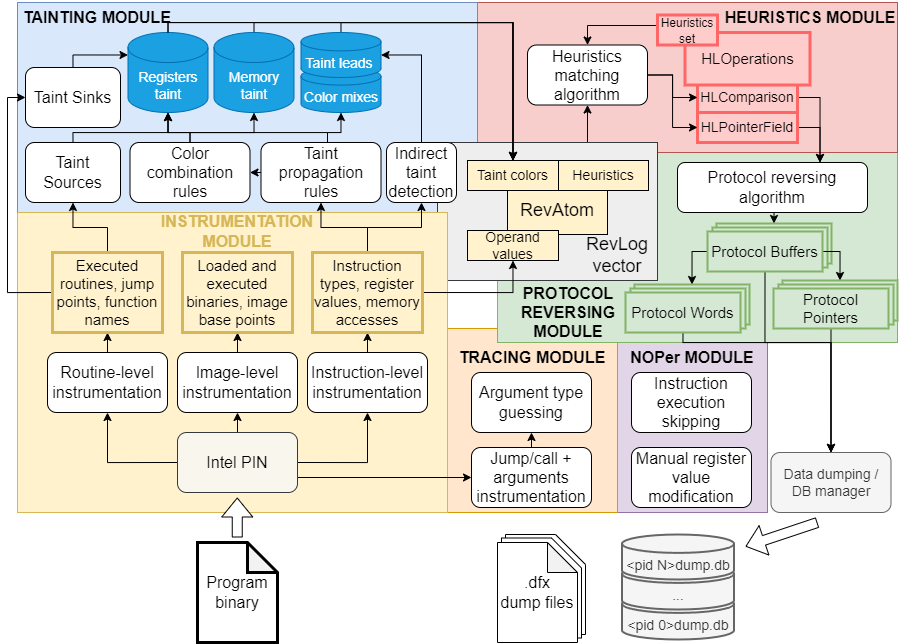
\includegraphics[width=\textwidth]{images/archdetailedsteps.drawio.png}}
    \caption{Example of a figure caption.}
    \label{fig_3_archdetailedsteps}
\end{figure*}

\subsection{Instrumentation module}
The instrumentation module is the central component in the \textit{TaintBlade} framework and the one 
that works at the lowest level. It utilizes Intel PIN to instrument the program that is being executed 
at a triple level: creating hooks for every loaded program image (e.g. an imported DLL), for every executed routine
(e.g. the \textit{main} function at the program) and for every executed instruction (e.g. a single call instruction to an
imported function). 

%\section{Implementation}
%NO - This section goes into detail on the algorithms implemented in the tool, including an overview of how the tainting
%engine works and how the heuristics engine and the protocol reversing engine on top work.

\section{Evaluation}
TODO - This section covers multiple test cases, including custom programs that
we will include in our repository that showcase some easy-to-understand cases
we want to show that work, and some others that are real malware found in the
wild.

Goal of the eval first. It's about checking functionality, and checking that we
detect e.g. all commands we know are at the sample

\section{Related work}
TODO decide whether to include this or not - It might fit better in the
background

\section{Conclusion}
TODO - This section offers an overview of the developed tool and the results
obtained over the problem we were trying to solve.

\subsection{Future work \& limitations}

\section*{Acknowledgment}
TODO

\begin{thebibliography}{00}
    \bibitem{b1} G. Eason, B. Noble, and I. N. Sneddon, ``Sample title,'' Phil. Trans. Roy. Soc. London, vol. A247, pp. 529--551, April 1955.
\end{thebibliography}
\vspace{12pt}

\end{document}

\appendix{}